% ACCESS-AIS3 overview talk (~20 min, broad climate audience). Same content as the web deck.
% Build: pdflatex ais3_overview.tex (twice). Speaker notes: uncomment the show notes line below.
\documentclass[aspectratio=169,11pt]{beamer}
% \setbeameroption{show notes on second screen=right}

\usepackage[T1]{fontenc}
\usepackage[utf8]{inputenc}
\usepackage{lmodern}
\usepackage{tgheros}
\renewcommand{\familydefault}{\sfdefault}
\usepackage{graphicx}
\usepackage{xcolor}
\usepackage{colortbl}
\usepackage{ragged2e}
\AtBeginDocument{\RaggedRight}
\graphicspath{{figs/}}

% ---- palette (as the web deck)
\definecolor{navy}{HTML}{14213D}
\definecolor{paper}{HTML}{FBFBF8}
\definecolor{paper2}{HTML}{EEF1EF}
\definecolor{ink}{HTML}{1F2A37}
\definecolor{muted}{HTML}{3D4A5C}
\definecolor{faint}{HTML}{5A6676}
\definecolor{accent}{HTML}{B4410E}
\definecolor{blue}{HTML}{1D5FA8}
\definecolor{green}{HTML}{0F7A5C}
\definecolor{sand}{HTML}{F4A261}
\definecolor{mist}{HTML}{B8C4D6}
\definecolor{cream}{HTML}{F3F1EA}

\newcommand{\serif}{\fontfamily{qpl}\selectfont}  % TeX Gyre Pagella for headings

% ---- beamer look
\setbeamertemplate{navigation symbols}{}
\setbeamercolor{background canvas}{bg=paper}
\setbeamercolor{normal text}{fg=ink}
\setbeamersize{text margin left=10mm, text margin right=10mm}
\setbeamertemplate{frametitle}{%
  \vspace*{5mm}%
  {\scriptsize\bfseries\color{accent}\MakeUppercase{\insertframesubtitle}}\par\vspace{1mm}%
  {\serif\Large\bfseries\color{navy}\hyphenpenalty=10000\insertframetitle\par}}
\setbeamertemplate{footline}{%
  \hbox to \paperwidth{\hspace{10mm}{\tiny\color{faint}\insertshortsource}\hfill
  {\tiny\color{faint}\insertframenumber}\hspace{10mm}}\vspace{4mm}}
\makeatletter
\newcommand{\insertshortsource}{\beamer@shortsource}
\newcommand{\source}[1]{\gdef\beamer@shortsource{#1}}
\gdef\beamer@shortsource{}
\makeatother
\newcommand{\nosource}{\source{}}

% card: width, background, headline colour, headline, body
\newcommand{\card}[5]{%
  \colorbox{#2}{\begin{minipage}[t][#1][t]{\dimexpr\linewidth-2\fboxsep\relax}
  \raggedright\vspace{2mm}{\serif\large\bfseries\color{#3}#4}\par\vspace{1.5mm}
  {\small\color{muted}#5}\vspace{2mm}\end{minipage}}}
% stat: number colour, number, caption
\newcommand{\stat}[3]{{\serif\Large\bfseries\color{#1}#2}\par\vspace{0.5mm}{\small\color{muted}#3}\par\vspace{4mm}}

\title{ACCESS-AIS3}
\author{Justin Hew \and Felicity McCormack}
\institute{ACCESS-NRI}
\date{ACCESS-NRI Cryosphere Workshop}

\begin{document}

% ============================================================ cover
{\setbeamercolor{background canvas}{bg=navy}
\setbeamertemplate{footline}{}
\begin{frame}
\vfill
{\scriptsize\bfseries\color{sand}ACCESS-NRI \textperiodcentered{} ANTARCTIC ICE SHEET}\par\vspace{4mm}
{\serif\fontsize{40}{44}\selectfont\bfseries\color{cream}ACCESS-AIS3}\par\vspace{5mm}
\begin{minipage}{0.8\linewidth}\large\color{mist}
An Antarctic ice-sheet model for ACCESS: how it is built, how well it matches today, and what it projects to 2300
\end{minipage}
\vfill
{\small\color{mist}Justin Hew \textperiodcentered{} Felicity McCormack \textperiodcentered{} ACCESS-NRI Cryosphere Workshop}
\vspace{6mm}
\note{Introduce yourself. AIS3 is the Antarctic ice-sheet configuration we are building for ACCESS. Today: what it is, whether it matches the observed ice sheet, and what it says about Antarctica's sea-level contribution out to 2300.}
\end{frame}}

% ============================================================ about
\nosource
\begin{frame}{An open, community model of the whole Antarctic ice sheet, built to run inside ACCESS}
\framesubtitle{What AIS3 is}
\vspace{0mm}
\begin{columns}[T]
\column{0.48\textwidth}
\card{18mm}{paper2}{accent}{Open}{Public configuration, inputs and workflow that anyone can rerun, check and extend}\par\vspace{3mm}
\card{18mm}{paper2}{navy}{Whole Antarctica}{Every ice stream, ice shelf and grounding line of the continent in one ISSM setup}
\column{0.48\textwidth}
\card{18mm}{paper2}{blue}{Community}{A shared starting point for Antarctic ice-sheet research, open to contributions}\par\vspace{3mm}
\card{18mm}{paper2}{green}{Built for ACCESS}{Designed from the start to plug into the ACCESS suite of climate models}
\end{columns}
\vspace{2mm}
{\small\color{muted}Code, configuration and workflow: \href{https://github.com/ACCESS-NRI/ACCESS-AIS3}{\bfseries\color{blue}github.com/ACCESS-NRI/ACCESS-AIS3}}
\note{AIS3 is a model configuration, not a new ice-sheet code: it uses ISSM and adds everything needed to run the whole Antarctic ice sheet: mesh, initial state, friction and rheology from inversions, ocean-melt calibration, forcing pipelines and the run workflow. Open and community-oriented so others can use it, check it and build on it. Everything is at github.com/ACCESS-NRI/ACCESS-AIS3: point people there if they want to run it.}
\end{frame}

% ============================================================ roadmap
\newcommand{\step}[5]{% background, label colour, label, title, body (title/body colours follow the background)
  \colorbox{#1}{\begin{minipage}[t][37mm][t]{\dimexpr\linewidth-2\fboxsep\relax}\raggedright\vspace{2mm}
  {\scriptsize\bfseries\color{#2}#3}\par\vspace{1mm}{\serif\large\bfseries#4}\par\vspace{1.5mm}{\small #5}\end{minipage}}}
\begin{frame}{AIS3 is designed to become the Antarctic ice sheet in the upcoming ACCESS-ESM3}
\framesubtitle{Where it is going}
\vspace{8mm}
\begin{columns}[c]
\column{0.29\textwidth}\step{paper2}{blue}{TODAY}{\color{navy}Standalone}{\color{muted}Forced by CMIP6 output under ISMIP protocols; results go to LARMIP-3 and ISMIP7}
\column{0.04\textwidth}\centering{\Large\color{mist}$\rightarrow$}
\column{0.29\textwidth}\step{paper2}{accent}{NEXT}{\color{navy}Coupling}{\color{muted}Exchange melt and meltwater with ACCESS's ocean; a GPU solver for coupled-run speed}
\column{0.04\textwidth}\centering{\Large\color{mist}$\rightarrow$}
\column{0.29\textwidth}\step{navy}{sand}{THEN}{\color{cream}ACCESS-ESM3}{\color{mist}An interactive Antarctic ice sheet inside ACCESS's next Earth system model}
\end{columns}
\note{Today AIS3 runs on its own, driven by climate-model output following the ISMIP protocols, and contributes to LARMIP-3 and ISMIP7. Next is coupling, so ice-shelf melt and meltwater respond to ACCESS's ocean rather than fixed forcing files; the GPU solver work makes coupled runs affordable. The target is the upcoming ACCESS-ESM3, where AIS3 is designed to be the interactive Antarctic ice sheet. Everything that follows in this talk is from the standalone stage. [Add a timeline for ESM3 integration if you want to commit to one.]}
\end{frame}

% ============================================================ why
\nosource
\begin{frame}{Antarctica holds the most ice, and the biggest uncertainty in long-term sea-level rise}
\framesubtitle{Why it matters}
\vspace{6mm}
\begin{columns}[T]
\column{0.32\textwidth}\card{38mm}{paper2}{accent}{\Huge $\sim$58 m}{of global sea level is stored in the Antarctic ice sheet}
\column{0.32\textwidth}\card{38mm}{paper2}{blue}{\LARGE Two forces}{More snowfall adds ice. A warmer ocean thins the floating ice shelves that hold the ice sheet back.}
\column{0.32\textwidth}\card{38mm}{paper2}{navy}{\LARGE No ice sheet}{in ACCESS yet. AIS3 is the first step towards one that runs with the climate model.}
\end{columns}
\note{About 58 m of sea-level equivalent (BedMachine Antarctica). Which of the two forces wins decides whether Antarctica adds to or offsets sea-level rise, and the balance is very uncertain beyond 2100. ACCESS has no interactive ice sheet; AIS3 is a standalone configuration driven by climate-model output, built so it can later be coupled.}
\end{frame}

% ============================================================ model
\begin{frame}{AIS3 runs the whole continent in ISSM, forced by climate-model output}
\framesubtitle{The model}
\vspace{4mm}
\begin{columns}[T]
\column{0.48\textwidth}
\card{21mm}{paper2}{navy}{Mesh}{1.59 million points over grounded ice, ice shelves and an ocean buffer}\par\vspace{3mm}
\card{21mm}{paper2}{navy}{Climate forcing}{Ocean temperature and snowfall minus melt from CMIP6 models, ISMIP6/7 protocol}
\column{0.48\textwidth}
\card{21mm}{paper2}{navy}{Ice flow, two ways}{SSA: 2D and fast, the main runs. HO: full 3D, 15 layers, used as a check.}\par\vspace{3mm}
\card{21mm}{paper2}{navy}{Runs}{Historical 1995--2019, then projections 2019--2300, on NCI's Gadi}
\end{columns}
\note{ISSM is the Ice-sheet and Sea-level System Model. SSA is the shallow-shelf approximation: depth-averaged and cheap. HO is the higher-order Blatter-Pattyn model: resolves vertical shear, about 15 times more points. Forcing follows ISMIP6/ISMIP7: ocean thermal forcing drives shelf melt through a calibrated parameterisation; surface mass balance comes from the climate model. [Add mesh resolution range if wanted.]}
\end{frame}

% ============================================================ fit
\source{Left: observed surface speed, MEaSUREs InSAR velocity v2 (Rignot et al., 2017). Right: model after the friction inversion. m/yr, log scale.}
\begin{frame}{We infer the friction under the ice so modelled flow matches satellite velocity}
\framesubtitle{Matching today}
\vspace{2mm}
\centering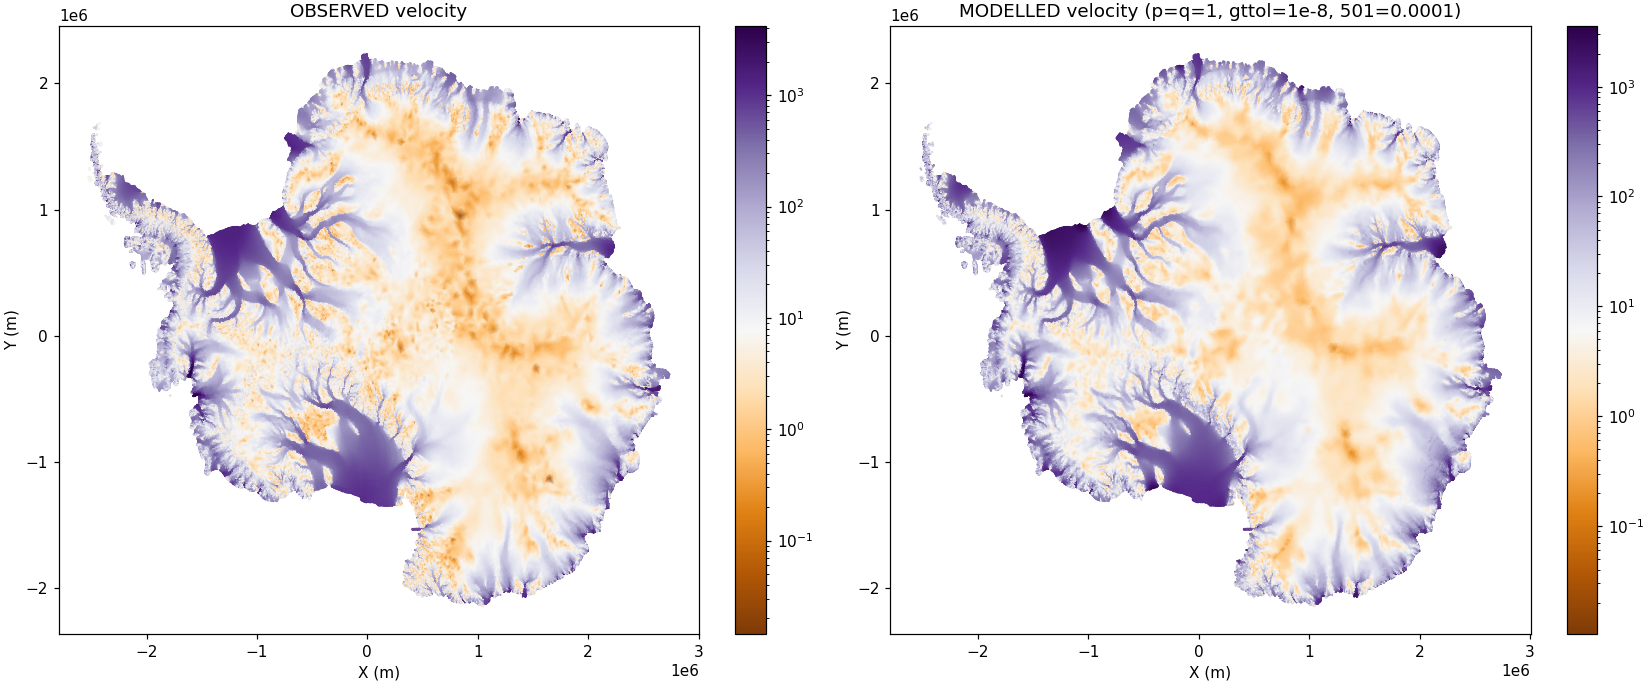
\includegraphics[height=0.62\textheight]{inversion.png}
\note{The friction at the bed can't be measured, so we solve for it: adjust friction until modelled surface speed matches the satellite velocity map. Fast ice streams (purple) and the slow interior (orange) are reproduced. Grounded-ice speed error in this inversion about 60 m/yr RMSE. [Check this figure is the friction field used in the final runs.]}
\end{frame}

% ============================================================ past
\source{Average dH/dt over grounded ice with satellite coverage every year. Black: CPOM radar altimetry (ISMIP7 MIPkit). Blue: SSA. Green: HO.}
\begin{frame}{From 1996 to 2019 the model tracks the year-to-year thinning and thickening seen by satellites}
\framesubtitle{Matching the recent past}
\vspace{1mm}
\centering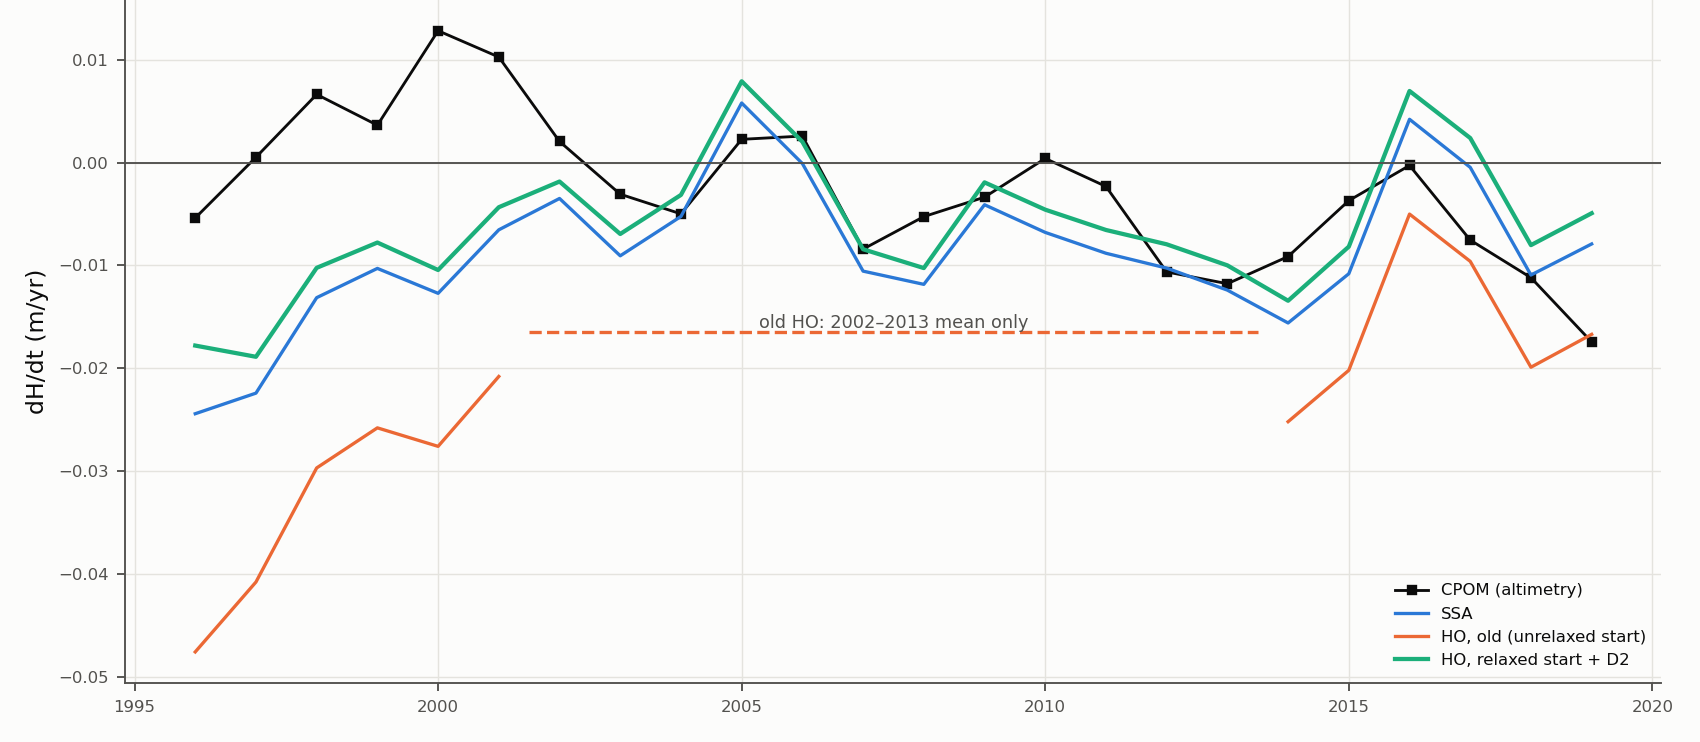
\includegraphics[height=0.6\textheight]{historical.png}
\note{Forced by historical climate, both model versions reproduce the interannual swings in thickness change measured by altimetry (CPOM), which are mostly snowfall-driven. The first few years are too negative: the model is still adjusting from its initial state. Orange is an earlier HO setup before we fixed its initial state and ice softness. SSA has the smallest error of the versions shown.}
\end{frame}

% ============================================================ future (statement)
{\setbeamercolor{background canvas}{bg=navy}
\setbeamertemplate{footline}{}
\begin{frame}
\vfill
{\scriptsize\bfseries\color{sand}PROJECTIONS TO 2300}\par\vspace{4mm}
\begin{minipage}{0.85\linewidth}
{\serif\LARGE\bfseries\color{cream}Under high emissions, Antarctica first gains ice for about 150 years, then loses it fast}\par\vspace{6mm}
{\color{mist}All numbers that follow are sea-level contribution relative to a constant-climate control run. Negative means Antarctica lowers sea level.}
\end{minipage}
\vfill
\note{Set up the sign convention before the plots: we always subtract a control run that keeps today's climate, so the numbers show the effect of climate change alone. Negative = the ice sheet gains mass and lowers sea level.}
\end{frame}}

% ============================================================ scenarios
\source{ACCESS-AIS3 (SSA), CESM2-WACCM forcing, minus control. Negative = sea-level fall.}
\begin{frame}{Low emissions lower sea level throughout; high emissions reverse after 2180}
\framesubtitle{Scenarios}
\begin{columns}[c]
\column{0.5\textwidth}\centering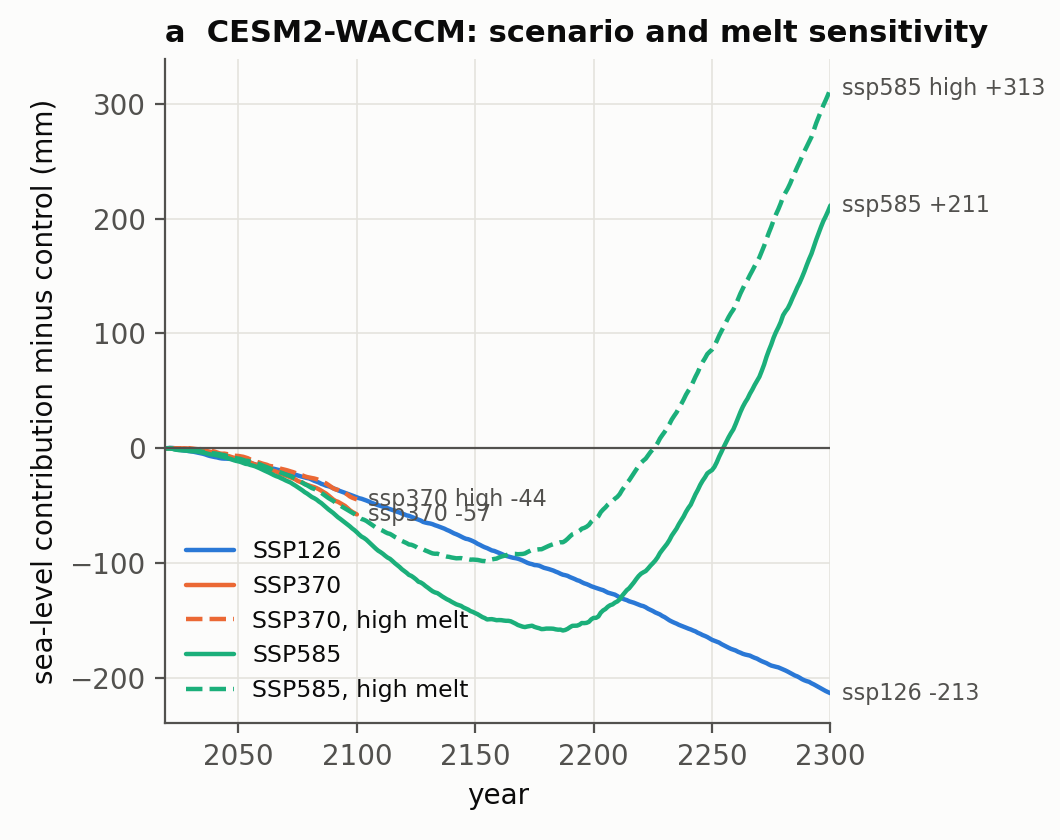
\includegraphics[height=0.62\textheight]{proj_scen.png}
\column{0.46\textwidth}
\stat{blue}{$-$213 mm}{SSP1-2.6 by 2300: a steady gain of ice}
\stat{green}{$-$160 $\rightarrow$ +211 mm}{SSP5-8.5: lowest near 2180, then a fast rise to 2300}
\stat{accent}{+313 mm}{SSP5-8.5 with high ocean melt}
\end{columns}
\note{One climate model (CESM2-WACCM) across three scenarios. SSP1-2.6: Antarctica keeps gaining mass for 280 years. SSP5-8.5: gains more at first, bottoms out around 2180 at about -160 mm, then +211 mm by 2300 and still accelerating. The high-melt member adds about another 100 mm. SSP3-7.0 only to 2100 (-57 mm, -44 with high melt).}
\end{frame}

% ============================================================ drivers
\source{SSP5-8.5, CESM2-WACCM. Separate runs with only ocean or only surface forcing, each minus control.}
\begin{frame}{The surface (snowfall minus melt) drives both the gain and the reversal}
\framesubtitle{What drives it}
\begin{columns}[c]
\column{0.44\textwidth}\centering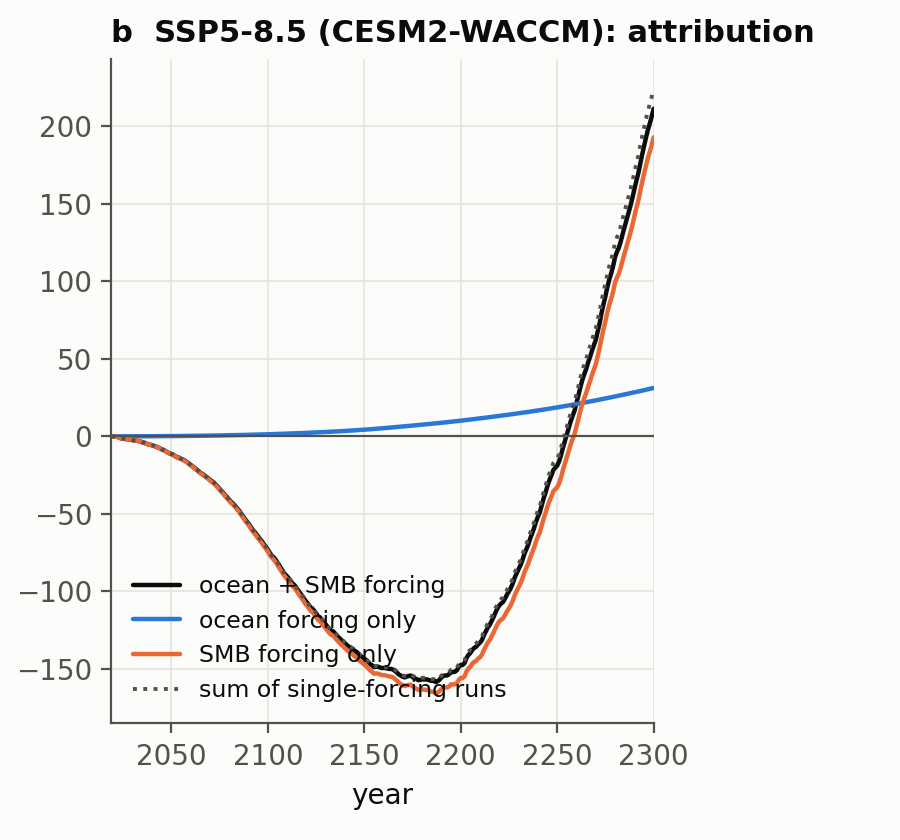
\includegraphics[height=0.62\textheight]{proj_attr.png}
\column{0.52\textwidth}
\stat{accent}{Surface only}{reproduces almost the whole response, dip and rise}
\stat{blue}{+31 mm}{from ocean melt alone by 2300, a slow and steady loss}
\stat{navy}{They add up}{the two single-forcing runs sum to the full run}
\end{columns}
\note{The high-emissions scenario run three ways: both forcings, ocean only, surface only. Almost all the response comes from surface mass balance: more snowfall early, then the surface balance turns against the ice. [Confirm the mechanism for the post-2180 reversal: increased surface melt and runoff in CESM2-WACCM.] Ocean melt adds only about 31 mm by 2300 in this model; we'll come back to why that is low.}
\end{frame}

% ============================================================ gcms
\source{ACCESS-AIS3 (SSA), reference melt, minus control. Negative = sea-level fall.}
\begin{frame}{Which climate model drives the ice sheet nearly doubles the 2100 answer}
\framesubtitle{Climate-model spread}
\begin{columns}[c]
\column{0.5\textwidth}\centering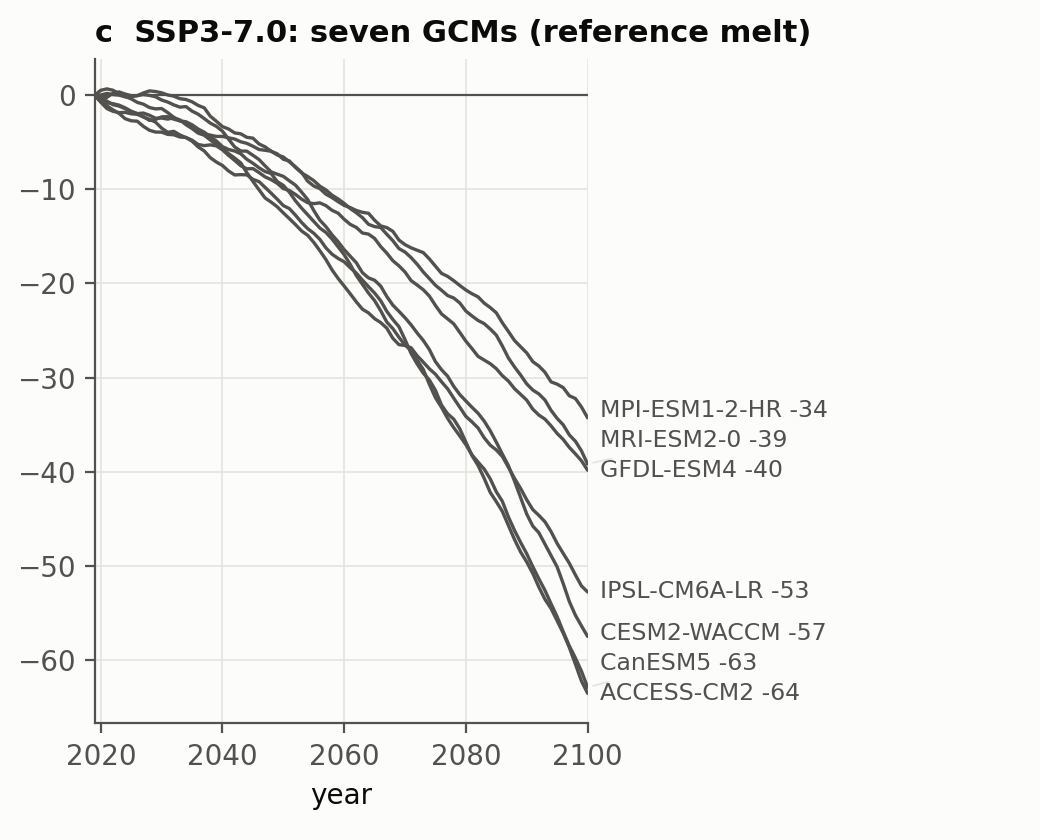
\includegraphics[height=0.62\textheight]{proj_gcm.png}
\column{0.46\textwidth}
\stat{blue}{$-$34 to $-$64 mm}{by 2100 across seven CMIP6 models, SSP3-7.0}
\stat{navy}{All negative}{every model adds snowfall faster than the ocean removes ice this century}
\stat{accent}{ACCESS-CM2}{gives the largest gain of the seven: $-$64 mm}
\end{columns}
\note{Same ice-sheet model, same scenario, seven climate models: almost a factor of two by 2100, from -34 mm (MPI-ESM1-2-HR) to -64 mm (ACCESS-CM2). These runs stop at 2100, so they don't show whether the late reversal seen with CESM2-WACCM happens with the other models too.}
\end{frame}

% ============================================================ collapse
\source{SSP5-8.5, CESM2-WACCM. ISMIP7 collapse mask (fracture path C, v2.1), applied every 1 January.}
\begin{frame}{If the ice shelves break up, sea level rises 315 mm more by 2300}
\framesubtitle{Ice-shelf collapse}
\vspace{1mm}
\centering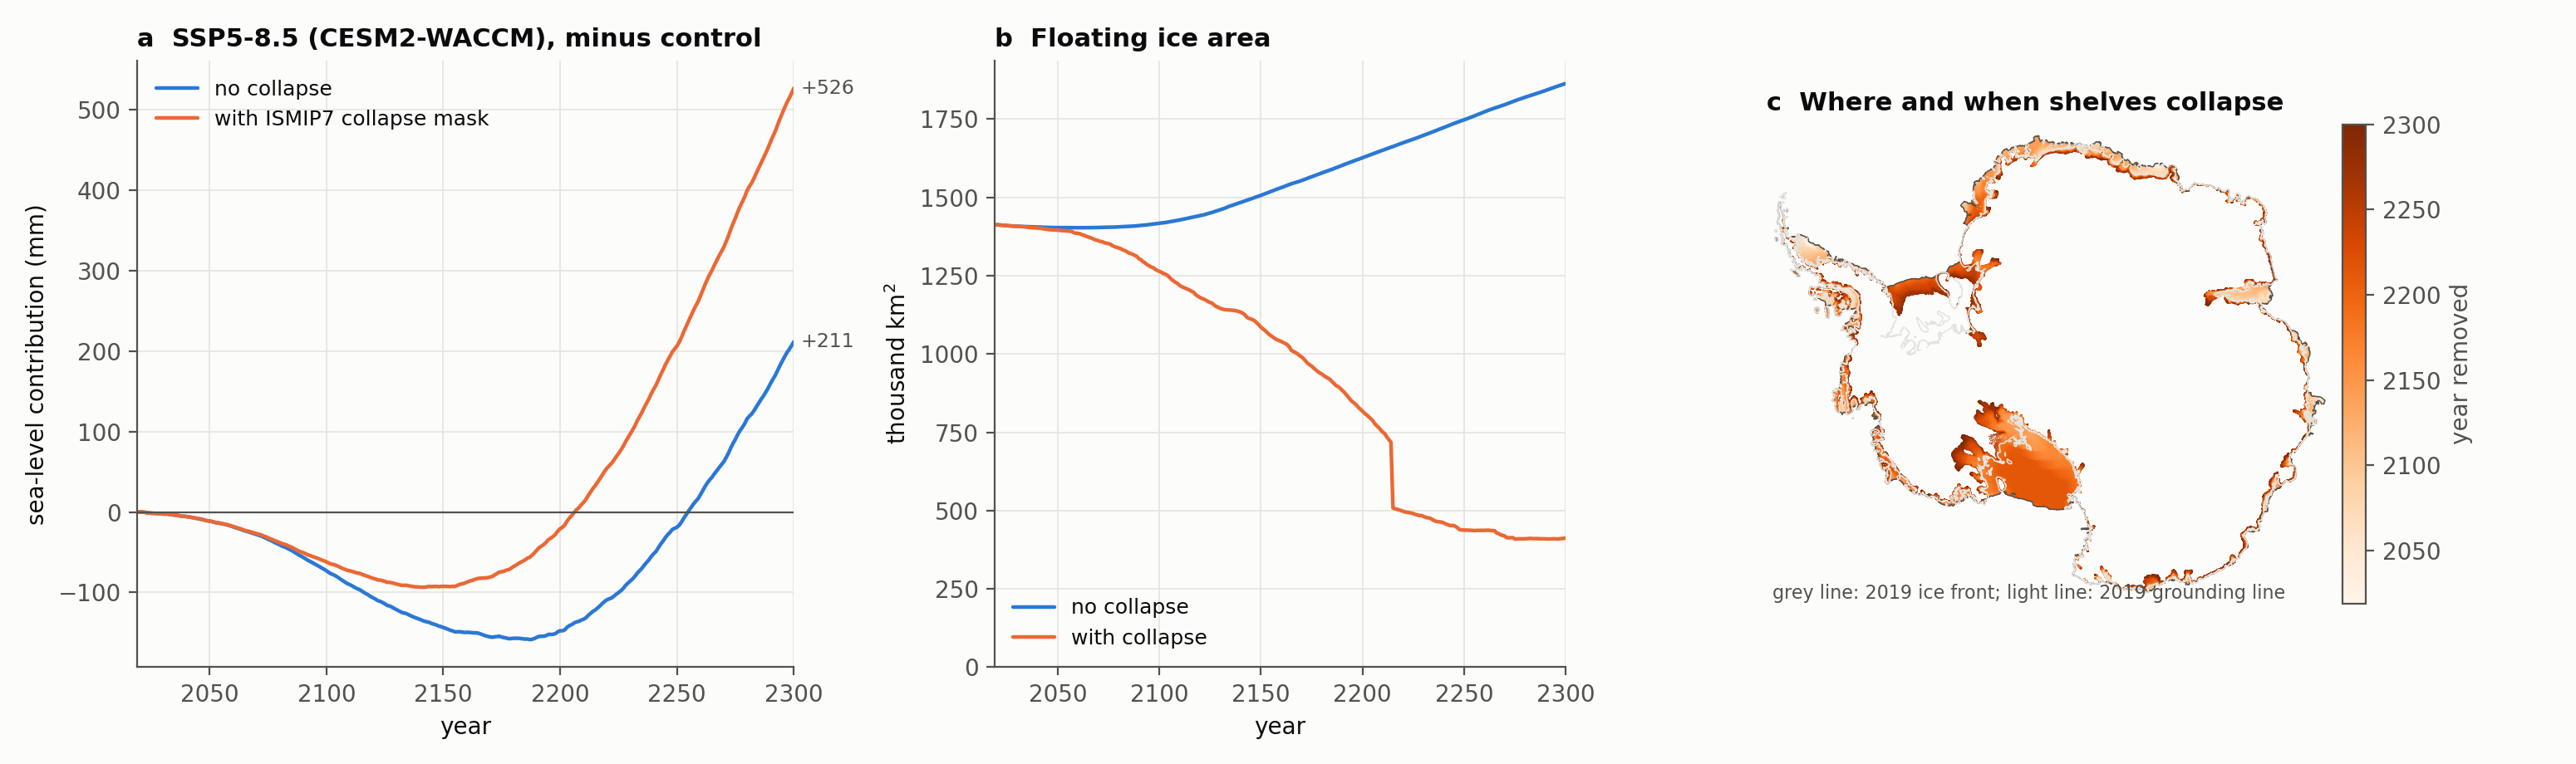
\includegraphics[width=0.86\linewidth]{collapse.png}\par\vspace{1mm}
\raggedright
\begin{columns}[T]
\column{0.48\textwidth}{\color{muted}\textbf{\color{accent}+526 mm} with collapse, against +211 mm without, by 2300}
\column{0.48\textwidth}{\color{muted}\textbf{\color{accent}2214:} most of the Ross Ice Shelf goes in a single year}
\end{columns}
\note{ISMIP7 provides a yearly map of where ice shelves are expected to break up from surface melt under warming. We remove that floating ice every January, plus any ice left with nothing holding it in place. Floating area drops from about 1.4 to 0.4 million km2. Without the shelves, grounded ice flows faster: an extra 315 mm by 2300. The step in 2214 is most of the Ross Ice Shelf at once. This is the biggest lever in our results, and it is a prescribed scenario, not a prediction.}
\end{frame}

% ============================================================ larmip
\source{Other models: LARMIP-2 (Levermann et al., 2020).}
\begin{frame}{AIS3 responds weakly to extra shelf melt compared with other ice-sheet models}
\framesubtitle{Sensitivity}
\vspace{1mm}
\centering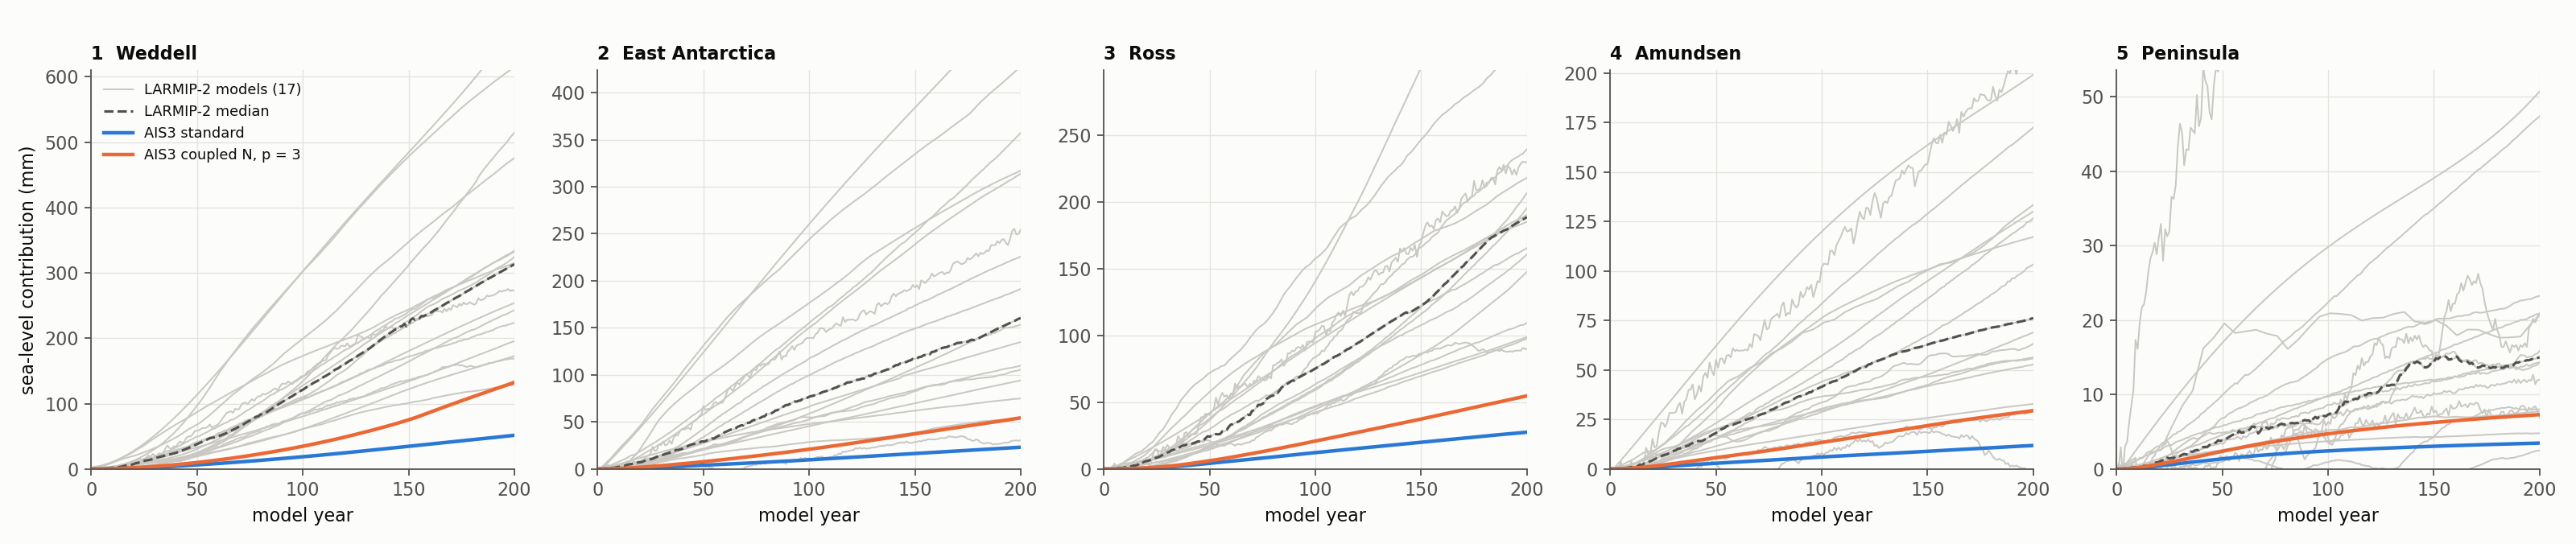
\includegraphics[width=\linewidth]{larmip.png}\par\vspace{3mm}
\raggedright
\begin{columns}[T]
\column{0.32\textwidth}\card{17mm}{paper2}{blue}{4--7$\times$ lower}{than the LARMIP-2 median after 200 years}
\column{0.32\textwidth}\card{17mm}{paper2}{accent}{2--3.5$\times$ lower}{with pressure-dependent, nonlinear sliding}
\column{0.32\textwidth}\card{17mm}{paper2}{navy}{About $\times$1.3}{more from melt at the grounding line}
\end{columns}
\note{LARMIP: every model gets the same extra 8 m/yr of melt under the shelves of one region. AIS3 (blue) sits near the bottom of the LARMIP-2 models in every region, 4-7 times below their median after 200 years. Friction that drops as the ice thins towards flotation, with nonlinear sliding (orange), roughly doubles to triples the response. Melt at the grounding line adds about 30\%. Together that closes about half the gap; candidates for the rest are high inverted friction near the grounding line, resolution and the SSA approximation. LARMIP-3 results were submitted in October 2026.}
\end{frame}

% ============================================================ HO vs SSA
\nosource
\begin{frame}{The 3D model agrees to 2100, then turns to ice loss sooner}
\framesubtitle{A check with full 3D flow}
\vspace{1mm}
\centering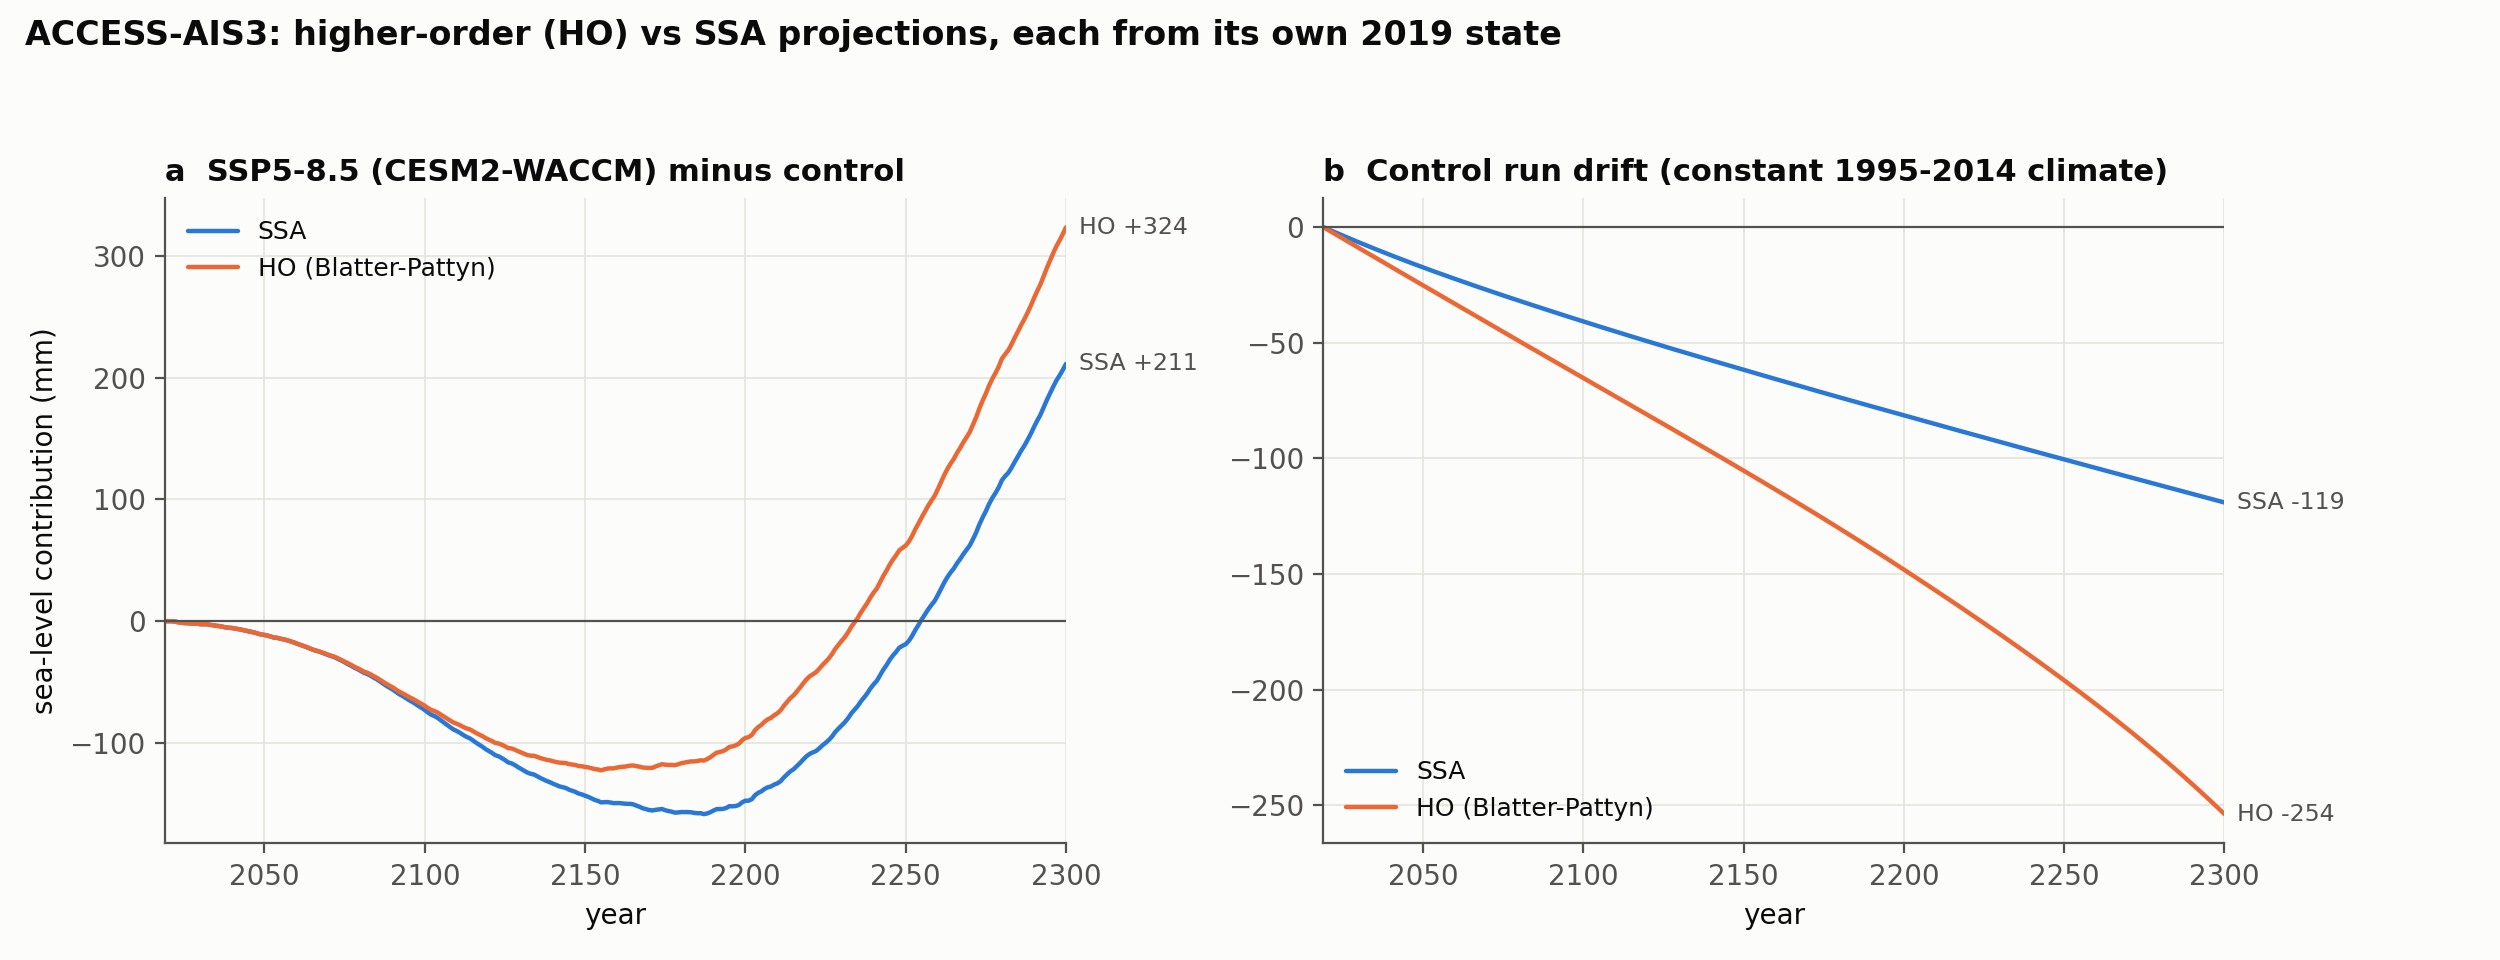
\includegraphics[height=0.47\textheight]{ho_vs_ssa_2300.png}\par\vspace{2mm}
\raggedright
\begin{columns}[T]
\column{0.48\textwidth}{\small\color{muted}\textbf{\color{blue}$-$70 vs $-$73 mm} by 2100; \textbf{\color{blue}+324 vs +211 mm} by 2300 (HO vs SSA, SSP5-8.5)}
\column{0.48\textwidth}{\small\color{muted}\textbf{\color{accent}Caveat:} HO friction only partly re-inverted, 8\% of grounded ice held at observed speed, control drifts twice as fast}
\end{columns}
\note{HO resolves the vertical structure of the flow and is about 15 times more expensive. From its own 2019 state, its response to SSP5-8.5 matches SSA within 5\% to 2100. After that HO gains less ice, turns to net loss around 2235 instead of 2255, and is 324 mm against 211 mm by 2300. Do not read the post-2200 gap as pure 3D physics: HO starts from the SSA friction with only a partial HO re-inversion, its ice-shelf stiffness comes from an earlier rheology inversion than SSA's, its control run gains ice about twice as fast, and to keep it stable we hold velocity at observed values on about 8\% of grounded ice, much of it near the Ross grounding line. HO is a check on the approximation, not a replacement for the SSA projections.}
\end{frame}

% ============================================================ takeaways
\nosource
{\setbeamercolor{background canvas}{bg=paper2}
\begin{frame}{Three things AIS3 tells us so far}
\framesubtitle{What it means}
\vspace{6mm}
\begin{columns}[T]
\column{0.32\textwidth}\card{36mm}{paper}{blue}{This century, snowfall wins}{Every scenario and climate model lowers sea level to 2100, by 34 to 73 mm.}
\column{0.32\textwidth}\card{36mm}{paper}{accent}{After 2180, it can flip}{High emissions give +211 mm by 2300, and +526 mm if the ice shelves break up.}
\column{0.32\textwidth}\card{36mm}{paper}{navy}{The ice may be too stable}{AIS3 reacts weakly to shelf loss, so its sea-level rise is likely on the low side.}
\end{columns}
\note{(1) To 2100 the extra snowfall outweighs ocean melt in every run we have. (2) Under high emissions that reverses, and shelf collapse more than doubles the 2300 number. (3) Our model is at the insensitive end of the ice-sheet model range, so treat the rises as conservative.}
\end{frame}}

% ============================================================ use: notebooks
\newcommand{\stage}[4]{% background, number colour, number, label colour+text
\colorbox{#1}{\begin{minipage}[t][16mm][t]{\dimexpr\linewidth-2\fboxsep\relax}\raggedright\vspace{1.5mm}
{\scriptsize\bfseries\color{#2}#3}\par\vspace{1mm}{\scriptsize\bfseries #4}\end{minipage}}}
\newcommand{\sarrow}{\column{0.018\textwidth}\centering{\color{mist}\scriptsize$\rightarrow$}}
\source{19 notebooks for the full 3D (HO) pipeline, plus 5 for the faster SSA track that starts from the same inversions.}
\begin{frame}{Every step of the pipeline is a notebook you can read and run}
\framesubtitle{Use it}
\vspace{2mm}
\begin{columns}[c,onlytextwidth]
\column{0.15\textwidth}\stage{paper2}{blue}{00--02}{\color{navy}Domain, mesh}
\sarrow
\column{0.15\textwidth}\stage{paper2}{blue}{03--10}{\color{navy}Inversions}
\sarrow
\column{0.15\textwidth}\stage{paper2}{blue}{11--12}{\color{navy}Initial state}
\sarrow
\column{0.15\textwidth}\stage{paper2}{blue}{13--16}{\color{navy}3D setup, melt}
\sarrow
\column{0.15\textwidth}\stage{paper2}{blue}{17}{\color{navy}History 1995--2019}
\sarrow
\column{0.15\textwidth}\stage{navy}{sand}{18}{\color{cream}Projections}
\end{columns}
\vspace{3mm}
\begin{columns}[T,onlytextwidth]
\column{0.3\textwidth}{\color{blue}\rule{\linewidth}{1.2pt}}\par\vspace{1mm}{\serif\large\bfseries\color{blue}Built from the code}\par\vspace{1mm}{\small\color{muted}Generated from the production scripts, so a notebook never drifts from what the runs actually did}
\column{0.3\textwidth}{\color{accent}\rule{\linewidth}{1.2pt}}\par\vspace{1mm}{\serif\large\bfseries\color{accent}Explains itself}\par\vspace{1mm}{\small\color{muted}Each one lists what it reads and writes, what to check afterwards, and the known pitfalls}
\column{0.3\textwidth}{\color{green}\rule{\linewidth}{1.2pt}}\par\vspace{1mm}{\serif\large\bfseries\color{green}Two ways to run}\par\vspace{1mm}{\small\color{muted}Step through it in Jupyter, or submit it as a batch job with the one-line command in its header}
\end{columns}
\note{The whole workflow, from cutting the domain and building the mesh through the inversions, the 3D setup, the historical run and the projections, is a sequence of numbered notebooks. They are generated from the same driver scripts the production runs use, so they show exactly what was done, and each carries hand-written notes on prerequisites, checks and pitfalls. The SSA track reuses the upstream inversions and has its own five notebooks. You can step through one interactively or run it unattended as a PBS job.}
\end{frame}

% ============================================================ start: getting started
\nosource
\begin{frame}{Getting started on NCI's Gadi}
\framesubtitle{Use it}
\vspace{2mm}
\renewcommand{\arraystretch}{1.2}\small\hyphenation{ISMIP}
\begin{tabular}{@{}p{0.04\linewidth}p{0.2\linewidth}p{0.7\linewidth}@{}}
\arrayrulecolor{paper2}\hline
{\serif\Large\bfseries\color{accent}1} & {\serif\large\bfseries\color{navy}Get access} & {\color{muted}An NCI account and membership of vk83 (ISSM build), av17 (ACCESS-NRI cryosphere data pool) and au88 (\mbox{ISMIP} forcing)}\\\hline
{\serif\Large\bfseries\color{accent}2} & {\serif\large\bfseries\color{navy}Get the code} & {\color{muted}\colorbox{paper2}{\footnotesize\ttfamily\color{navy}git clone github.com/ACCESS-NRI/ACCESS-AIS3}, plus a Python environment with pyISSM}\\\hline
{\serif\Large\bfseries\color{accent}3} & {\serif\large\bfseries\color{navy}Run a step} & {\color{muted}Open its notebook, or \colorbox{paper2}{\footnotesize\ttfamily\color{navy}qsub -v AIS3\_STEPS=<step>} with its launcher. The run guide covers resources and known failures}\\\hline
\end{tabular}
\vspace{1mm}
\begin{columns}[T,onlytextwidth]
\column{0.48\textwidth}\colorbox{paper2}{\begin{minipage}{\dimexpr\linewidth-2\fboxsep\relax}\vspace{1mm}\footnotesize\color{muted}\textbf{\color{navy}Cost:} a 10-year HO projection chunk takes about 12\,h on 96 cores; the SSA track is far cheaper\vspace{1mm}\end{minipage}}
\column{0.48\textwidth}\colorbox{paper2}{\begin{minipage}{\dimexpr\linewidth-2\fboxsep\relax}\vspace{1mm}\footnotesize\color{muted}\textbf{\color{accent}One file to edit:} {\ttfamily\color{navy}config/site.env} sets your project, storage and Python; submit with {\ttfamily\color{navy}./submit}\vspace{1mm}\end{minipage}}
\end{columns}
\note{You need an NCI account and three projects: vk83 for ACCESS-NRI's ISSM build (the access-issm\_ad module), av17 for the cryosphere data pool the inputs are read from, and au88 for the ISMIP forcing. Clone the repository, set up a Python environment with pyISSM, then run steps from their notebooks or with qsub and the step's launcher; docs/run\_guide.md has resources, timings and known failures. Everything account-specific is in one file, config/site.env: NCI project, storage, Python environment, ISSM build and forcing location. Repository root and username are found automatically; ./submit is qsub with your project and storage filled in.}
\end{frame}

% ============================================================ next
\begin{frame}{Where AIS3 goes from here}
\framesubtitle{Next}
\vspace{3mm}
\renewcommand{\arraystretch}{1.3}\small
\begin{tabular}{@{}p{0.27\linewidth}p{0.66\linewidth}@{}}
\arrayrulecolor{paper2}\hline
{\serif\large\bfseries\color{navy}Couple to ACCESS} & {\color{muted}Run the ice sheet with ACCESS's ocean, so shelf melt and meltwater respond to each other}\\\hline
{\serif\large\bfseries\color{navy}Faster on GPUs} & {\color{muted}GPU solver: a one-year run 1.5$\times$ faster and 1.9$\times$ cheaper than 48 CPU cores}\\\hline
{\serif\large\bfseries\color{navy}Close the gap} & {\color{muted}Find why AIS3 reacts weakly to shelf loss: friction near the grounding line, resolution}\\\hline
{\serif\large\bfseries\color{navy}Publish} & {\color{muted}LARMIP-3 submitted; ISMIP7 runs and a model-description paper in progress}\\\hline
\end{tabular}
\note{Coupling: an ice sheet that runs inside ACCESS, exchanging melt and meltwater with the ocean model instead of reading fixed forcing files. GPU: ISSM with the hypre BoomerAMG solver on one A100 ran a one-year SSA transient 1.5x faster and with 1.9x fewer service units than the 48-core MUMPS direct solver, with the same answer. Sensitivity: about half of the gap to other models is explained. Papers: LARMIP-3 sent October 2026; a GMD-style model description paper is planned. [Adjust timelines to what you want to commit to publicly.]}
\end{frame}

% ============================================================ thanks
{\setbeamercolor{background canvas}{bg=navy}
\setbeamertemplate{footline}{}
\begin{frame}
\vfill
{\serif\fontsize{40}{44}\selectfont\bfseries\color{cream}Thank you}\par\vspace{4mm}
{\Large\color{sand}Questions?}\par\vspace{4mm}
{\color{mist}Justin Hew (ACCESS-NRI) \textperiodcentered{} Felicity McCormack}\par\vspace{2mm}
{\color{sand}\href{https://github.com/ACCESS-NRI/ACCESS-AIS3}{github.com/ACCESS-NRI/ACCESS-AIS3}}
\vfill
{\scriptsize\color{mist}Computing on NCI's Gadi. Ice-sheet model: ISSM. Forcing: CMIP6 via ISMIP6/ISMIP7. Data: MEaSUREs velocity, BedMachine v3, RACMO2.4p1, CPOM altimetry, Aq1, ISMIP7. Full list on the next slide.}
\vspace{6mm}
\note{Likely questions: why does Antarctica gain mass? (snowfall increase in a warmer atmosphere); how does this compare with IPCC? [prepare the AR6 Antarctic ranges you want to quote; our negative values come from the strong snowfall increase in these forcings and the model's low ice-shelf sensitivity]; is collapse realistic? (it is a prescribed ISMIP7 scenario).}
\end{frame}}

% ============================================================ references (backup)
\nosource
\begin{frame}{Data and references}
\framesubtitle{Backup}
\vspace{-1mm}\scriptsize\raggedright
\begin{columns}[T]
\column{0.52\textwidth}
{\bfseries\color{accent}Observations and inputs}\par\vspace{1.5mm}
\textbf{Ice velocity:} MEaSUREs InSAR velocity map v2. Rignot, Mouginot \& Scheuchl (2017), NSIDC.\par\vspace{0.8mm}
\textbf{Bed and thickness:} BedMachine Antarctica v3. Morlighem et al. (2020), \emph{Nat.\ Geosci.} 13, 132--137.\par\vspace{0.8mm}
\textbf{Coastline:} MEaSUREs Antarctic Boundaries. Mouginot et al. (2017), NSIDC.\par\vspace{0.8mm}
\textbf{SMB, surface temperature:} RACMO2.4p1. van Dalum et al. (2024), \emph{The Cryosphere} 18, 4065--4088.\par\vspace{0.8mm}
\textbf{Geothermal heat flow:} Aq1. St\aa l et al. (2021), \emph{G-cubed} 22, e2020GC009428.\par\vspace{0.8mm}
\textbf{Thickness change:} CPOM radar altimetry 1993--2019, from the ISMIP7 observations MIPkit v1.2.\par\vspace{0.8mm}
\textbf{Ocean:} ISMIP7 thermal-forcing climatology; IMBIE2 basins.
\column{0.44\textwidth}
{\bfseries\color{accent}Model and forcing}\par\vspace{1.5mm}
\textbf{Ice-sheet model:} ISSM. Larour et al. (2012), \emph{JGR Earth Surf.} 117, F01022.\par\vspace{0.8mm}
\textbf{Ocean melt:} ISMIP6 quadratic parameterisation. Jourdain et al. (2020), \emph{The Cryosphere} 14, 3111--3134.\par\vspace{0.8mm}
\textbf{Climate forcing:} CMIP6 (Eyring et al., 2016, \emph{GMD} 9, 1937--1958), incl.\ CESM2-WACCM (Gettelman et al., 2019), via the ISMIP6/ISMIP7 protocols.\par\vspace{0.8mm}
\textbf{Ice-shelf collapse:} ISMIP7 collapse masks (fracture path C, v2.1).\par\vspace{0.8mm}
\textbf{Melt sensitivity:} LARMIP-2. Levermann et al. (2020), \emph{Earth Syst.\ Dynam.} 11, 35--76.\par\vspace{0.8mm}
\textbf{Computing:} NCI Gadi.\par\vspace{3mm}
{\color{muted}Code: \href{https://github.com/ACCESS-NRI/ACCESS-AIS3}{github.com/ACCESS-NRI/ACCESS-AIS3}}
\end{columns}
\end{frame}

\end{document}
